%% 第4章 系统详细设计与实现

\chapter{系统详细设计与实现}

本章围绕论文确定的五个核心模块展开：用户认证与系统安全支撑、Agent 管理与可视化编排、
工作流调度执行、人工检查点与工作流恢复、知识库与检索增强。
同时，为了体现前后端实时联动效果，最后补充 SSE 全链路推流实现。
各功能模块均按照"实现过程 → 关键代码 → 界面展示"的结构进行描述。

\section{用户认证与系统安全支撑实现}

\subsection{注册、登录与密码找回流程}

\subsubsection{（1）实现过程}

用户认证模块是系统对外开放访问的基础支撑，主要围绕邮箱验证码、注册、登录与找回密码形成闭环。
系统在验证码发送前校验邮箱格式和发送频率，验证码写入缓存后通过邮件服务发送给用户。

注册时，系统校验验证码、密码强度以及邮箱和用户名唯一性，校验通过后使用 BCrypt 保存密码哈希；
登录时，系统根据邮箱查询用户并校验密码，失败时记录限流信息，成功后清理失败计数并交由接口层签发令牌。
找回密码流程复用验证码校验机制，在新密码符合强度要求后完成密码重置。

\subsubsection{（2）关键代码}

代码4-1展示了邮箱验证码发送、注册与登录的关键逻辑：

\begin{lstlisting}[language=Java, caption={代码4-1 UserAuthenticationDomainService -- 用户认证核心逻辑}]
public void sendVerificationCode(String emailStr) {
    Email email = Email.of(emailStr);
    validateEmailSendRateLimit(email);
    String code = generateSecureCode();
    verificationCodeRepository.save(email.getValue(), code, 5);
    emailService.sendVerificationCode(email, code);
}

public User register(String emailStr, String code, String password, String username) {
    Email email = Email.of(emailStr);
    validateVerificationCode(email, code);
    validatePasswordStrength(password);
    User user = User.create(email, Username.of(username), BCryptUtil.encode(password));
    userRepository.save(user);
    verificationCodeRepository.delete(email.getValue());
    return user;
}

public User login(String emailStr, String password, String ip) {
    checkLoginRateLimit(emailStr, ip);
    User user = userRepository.findByEmail(Email.of(emailStr)).orElseThrow();
    if (!BCryptUtil.matches(password, user.getPasswordHash())) {
        recordLoginFailure(emailStr, ip);
        throw new IllegalArgumentException("密码错误");
    }
    clearLoginFailures(emailStr, ip);
    return user;
}
\end{lstlisting}

代码4-2展示了异步邮件发送实现：

\begin{lstlisting}[language=Java, caption={代码4-2 EmailServiceImpl -- 验证码异步发送}]
@Override
public void sendVerificationCode(Email to, String code) {
    try {
        doSendAsync(to, code);
    } catch (Exception e) {
        throw new RuntimeException("发送验证码失败", e);
    }
}

@Async
public void doSendAsync(Email to, String code) {
    doSend(to, code);
}
\end{lstlisting}

\subsubsection{（3）界面展示}

前端提供登录、注册与忘记密码页面，用户通过邮箱验证码完成身份验证。
该模块保证了系统中的 Agent 管理、工作流执行、知识库管理等功能均运行在已认证用户上下文中。

\begin{figure}[H]
  \centering
  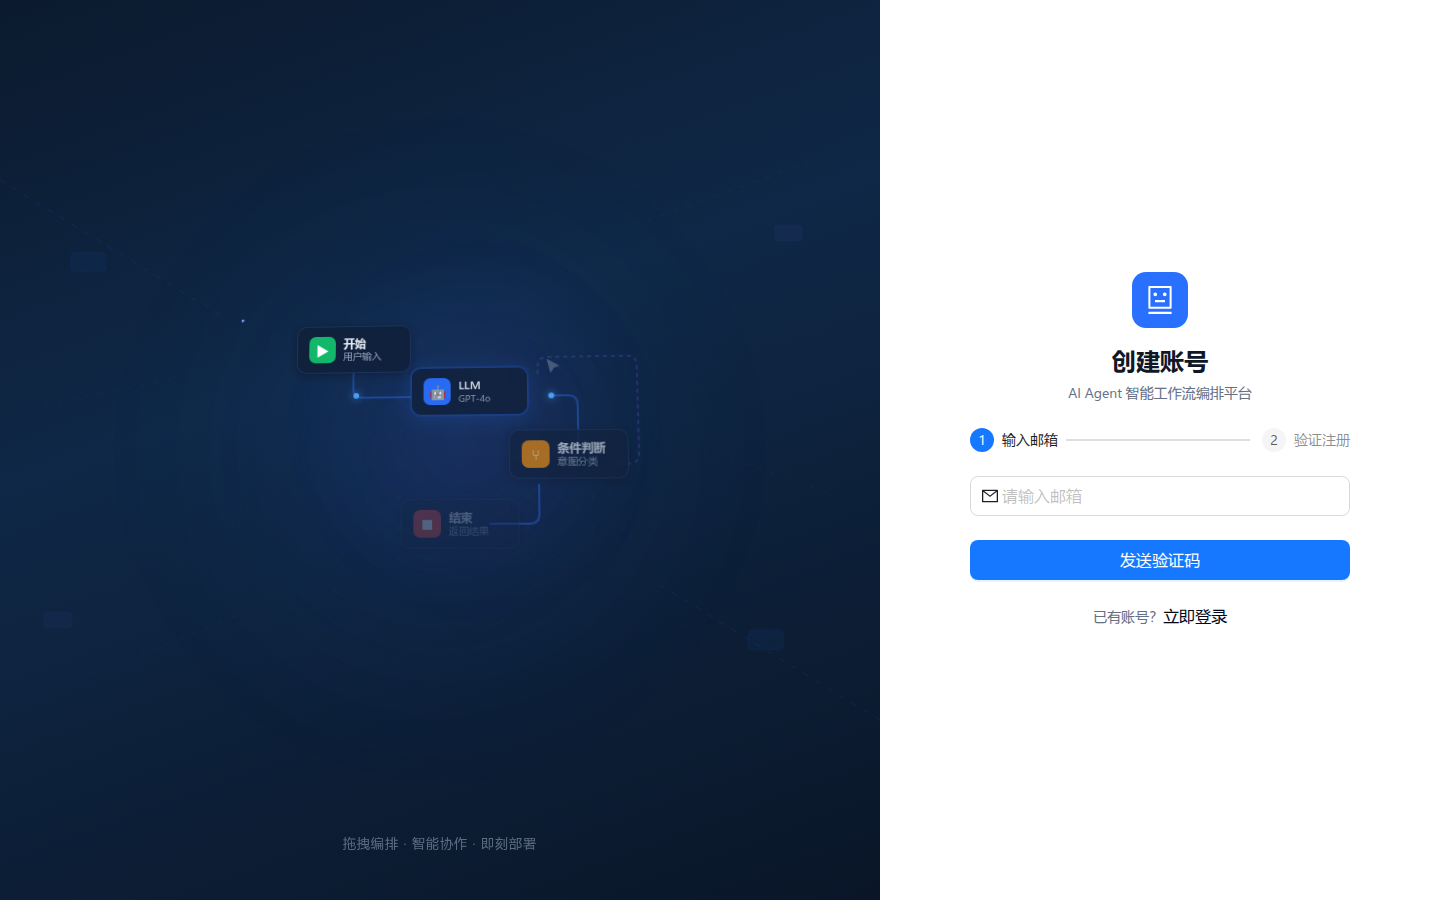
\includegraphics[width=0.85\textwidth]{figures/fig_auth_ui.png}
  \caption{用户认证界面}
  \label{fig:auth_ui}
\end{figure}

\subsection{安全控制机制}

\subsubsection{（1）实现过程}

除基本认证流程外，系统还通过多种机制加强访问安全与操作安全：

\begin{itemize}
  \item \textbf{验证码频率限制：}防止短时间内重复请求邮件验证码，降低接口滥用风险；
  \item \textbf{登录失败限流：}对同一邮箱或 IP 的连续失败登录进行限制，降低暴力破解风险；
  \item \textbf{密码加密存储：}使用 BCrypt 哈希算法保存密码，不在数据库中保留明文；
  \item \textbf{JWT 令牌认证：}用户登录成功后由接口层签发令牌，后续请求通过统一认证机制识别用户身份；
  \item \textbf{用户上下文隔离：}业务接口通过当前用户 ID 进行所有权校验，避免跨用户访问 Agent、知识库或执行记录。
\end{itemize}

这些安全能力并不直接产生业务结果，但构成了系统可被真实用户安全访问和使用的基础支撑层。

\section{Agent 管理与可视化编排实现}

\subsection{Agent 创建与版本管理}

\subsubsection{（1）实现过程}

Agent 管理模块承担工作流定义的生命周期管理职责，包括创建、修改、发布、回滚与版本查询。
用户创建 Agent 时，系统根据默认模板生成初始 \texttt{graphJson}；用户在 React Flow 画布中完成节点拖拽、参数配置和连线后，前端将新的图结构提交到后端保存为草稿。

当流程配置确认可用后，发布操作会结合图校验器生成 \texttt{AgentVersion} 快照；若后续需要恢复历史配置，系统可根据版本号读取快照并回滚当前 Agent。
该机制形成了"草稿编辑 → 发布快照 → 历史回滚"的版本管理链路，保证运行时图定义具备可追溯性。

\subsubsection{（2）关键代码}

代码4-3展示了 Agent 创建、更新、发布与回滚的核心逻辑：

\begin{lstlisting}[language=Java, caption={代码4-3 AgentApplicationService -- Agent 生命周期管理关键代码}]
@Transactional(rollbackFor = Exception.class)
public Long createAgent(CreateAgentCmd cmd) {
    String graphJson = generateInitialGraphJson();
    Agent agent = Agent.builder()
        .userId(cmd.getUserId())
        .name(cmd.getName())
        .graphJson(graphJson)
        .version(1)
        .build();
    agentRepository.save(agent);
    return agent.getId();
}

@Transactional(rollbackFor = Exception.class)
public void publishAgent(PublishAgentCmd cmd) {
    Agent agent = agentRepository.findById(cmd.getId()).orElseThrow();
    Integer nextVersion = agentRepository.findMaxVersion(agent.getId()).orElse(0) + 1;
    AgentVersion version = agent.publish(graphValidator, nextVersion);
    agentRepository.saveVersion(version);
    agent.setPublishedVersionId(version.getVersion().longValue());
    agentRepository.save(agent);
}
\end{lstlisting}

\subsubsection{（3）界面展示}

前端基于 React Flow 提供可视化画布，支持节点拖拽、参数配置、边连接与保存。
用户可在同一页面中完成 Agent 基础信息维护、流程图编辑以及版本发布操作。

\begin{figure}[H]
  \centering
  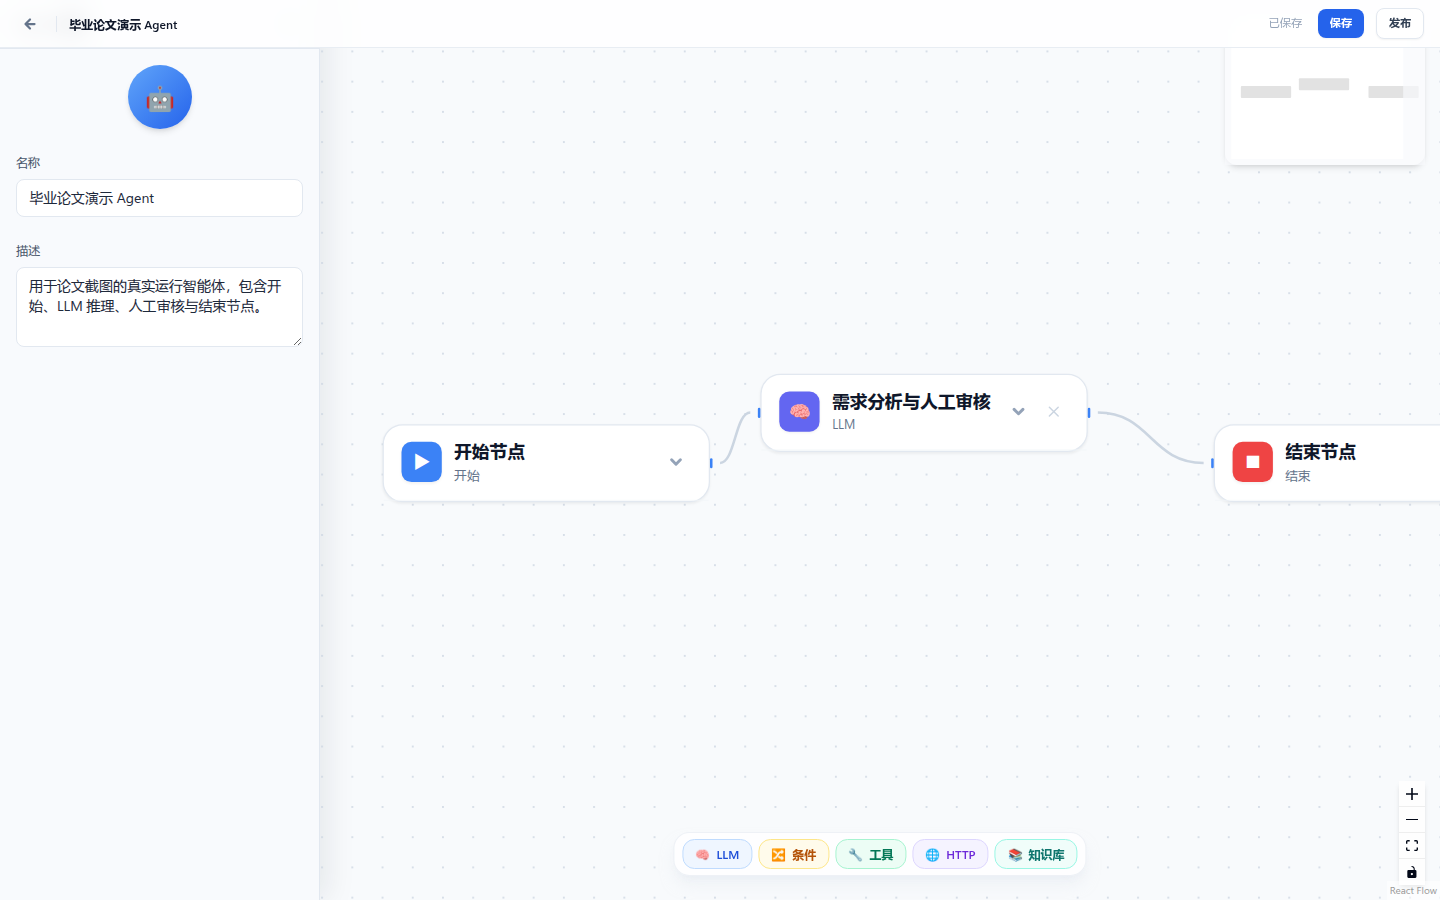
\includegraphics[width=0.95\textwidth]{figures/fig_agent_editor.png}
  \caption{Agent 可视化编排界面}
  \label{fig:agent_editor}
\end{figure}

\subsection{工作流图定义与运行时衔接}

\subsubsection{（1）实现过程}

Agent 可视化编排的最终结果并不是静态页面数据，而是运行时调度的直接输入。
当前端保存画布后，节点、边、节点参数等结构统一写入 \texttt{graphJson} 字段。
该字段既作为编辑态草稿保存，也可在发布后固化为版本快照。

工作流执行启动时，调度器首先根据 \texttt{agentId} 查询 Agent 实体。
若用户显式指定了 \texttt{versionId}，则优先读取对应 \texttt{AgentVersion} 的图定义；
否则优先加载已发布版本，若不存在再回退到当前草稿。随后，调度器通过
\texttt{WorkflowGraphFactoryImpl.fromJson()} 将 \texttt{graphJson} 反序列化为领域层的
\texttt{WorkflowGraph}，供后续 \texttt{Execution} 聚合根执行调度。

这一机制实现了可视化编排与运行时执行的直接衔接，使前端画布不只是配置界面，
而是工作流引擎的图定义来源。

\subsubsection{（2）关键代码}

代码4-4展示了调度器读取版本图定义并反序列化为工作流图的关键过程：

\begin{lstlisting}[language=Java, caption={代码4-4 SchedulerService -- graphJson 装载与工作流图解析}]
public void startExecution(String executionId, Long agentId, Long userId,
        String conversationId, Integer versionId,
        Map<String, Object> inputs, ExecutionMode mode) {
    Agent agent = agentRepository.findById(agentId).orElseThrow();

    String graphJson;
    if (versionId != null) {
        graphJson = agentRepository.findVersion(agentId, versionId)
            .orElseThrow().getGraphJson();
    } else if (agent.getPublishedVersionId() != null) {
        graphJson = agentRepository.findVersion(agentId,
            agent.getPublishedVersionId().intValue())
            .orElseThrow().getGraphJson();
    } else {
        graphJson = agent.getGraphJson();
    }

    WorkflowGraph graph = workflowGraphFactory.fromJson(graphJson);
    Execution execution = Execution.create(executionId, agentId, userId,
        conversationId, graph, mode);
    startExecution(execution, inputs, mode);
}
\end{lstlisting}

\subsubsection{（3）界面展示}

在 Agent 列表页中，用户可查看已创建的 Agent、进入编辑页继续修改，
也可查看已发布版本历史并执行回滚操作，实现从配置、发布到追踪的全流程管理。

\begin{figure}[H]
  \centering
  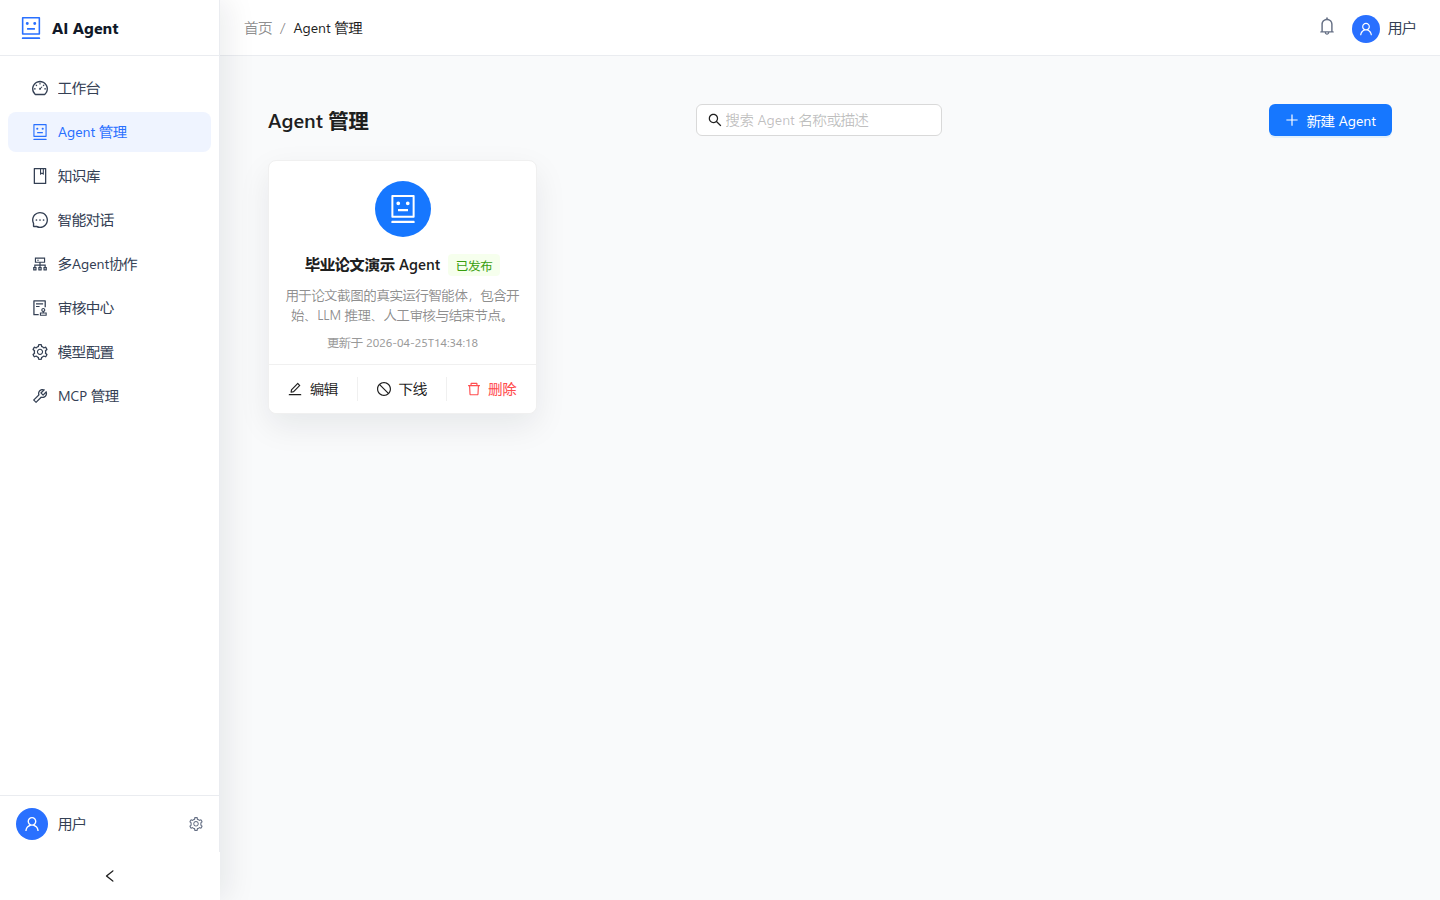
\includegraphics[width=0.9\textwidth]{figures/fig_agent_list.png}
  \caption{Agent 列表与版本管理界面}
  \label{fig:agent_list}
\end{figure}

\section{工作流调度执行实现}

\subsection{工作流执行启动模块}

\subsubsection{（1）实现过程}

工作流执行的启动入口位于应用层 \texttt{SchedulerService.startExecution()} 方法。
调度器根据 \texttt{agentId} 和可选 \texttt{versionId} 读取对应图定义，
再通过 \texttt{WorkflowGraphFactoryImpl.fromJson()} 将 JSON 配置转换为领域层 \texttt{WorkflowGraph}。

执行启动前，系统会向 \texttt{ExecutionContext} 注入会话历史和向量检索结果，随后调用
\texttt{Execution.start(inputs)} 完成 DAG 校验、节点状态初始化和首批就绪节点计算。
初始执行状态持久化后，调度器异步提交首批节点执行任务，工作流由此进入运行阶段。

\subsubsection{（2）关键代码}

代码4-5展示了工作流执行启动的核心逻辑（简化）：

\begin{lstlisting}[language=Java, caption={代码4-5 SchedulerService -- startExecution 启动流程关键代码}]
private void startExecution(Execution execution,
        Map<String, Object> inputs, ExecutionMode mode) {

    // 上下文增强：加载会话历史和检索结果
    hydrateMemory(execution, inputs);

    // 启动执行聚合根，获取首批就绪节点
    List<Node> readyNodes = execution.start(inputs);

    // 持久化初始状态并调度首批节点
    executionRepository.save(execution);
    scheduleNodes(execution.getExecutionId(), readyNodes, null);
}
\end{lstlisting}

\subsubsection{（3）界面展示}

前端在接收到工作流触发请求后，建立 SSE 连接，并实时展示各节点的执行进度。
节点蓝色高亮表示正在运行，绿色表示已完成，灰色表示已跳过（条件分支未选中路径）。

\begin{figure}[H]
  \centering
  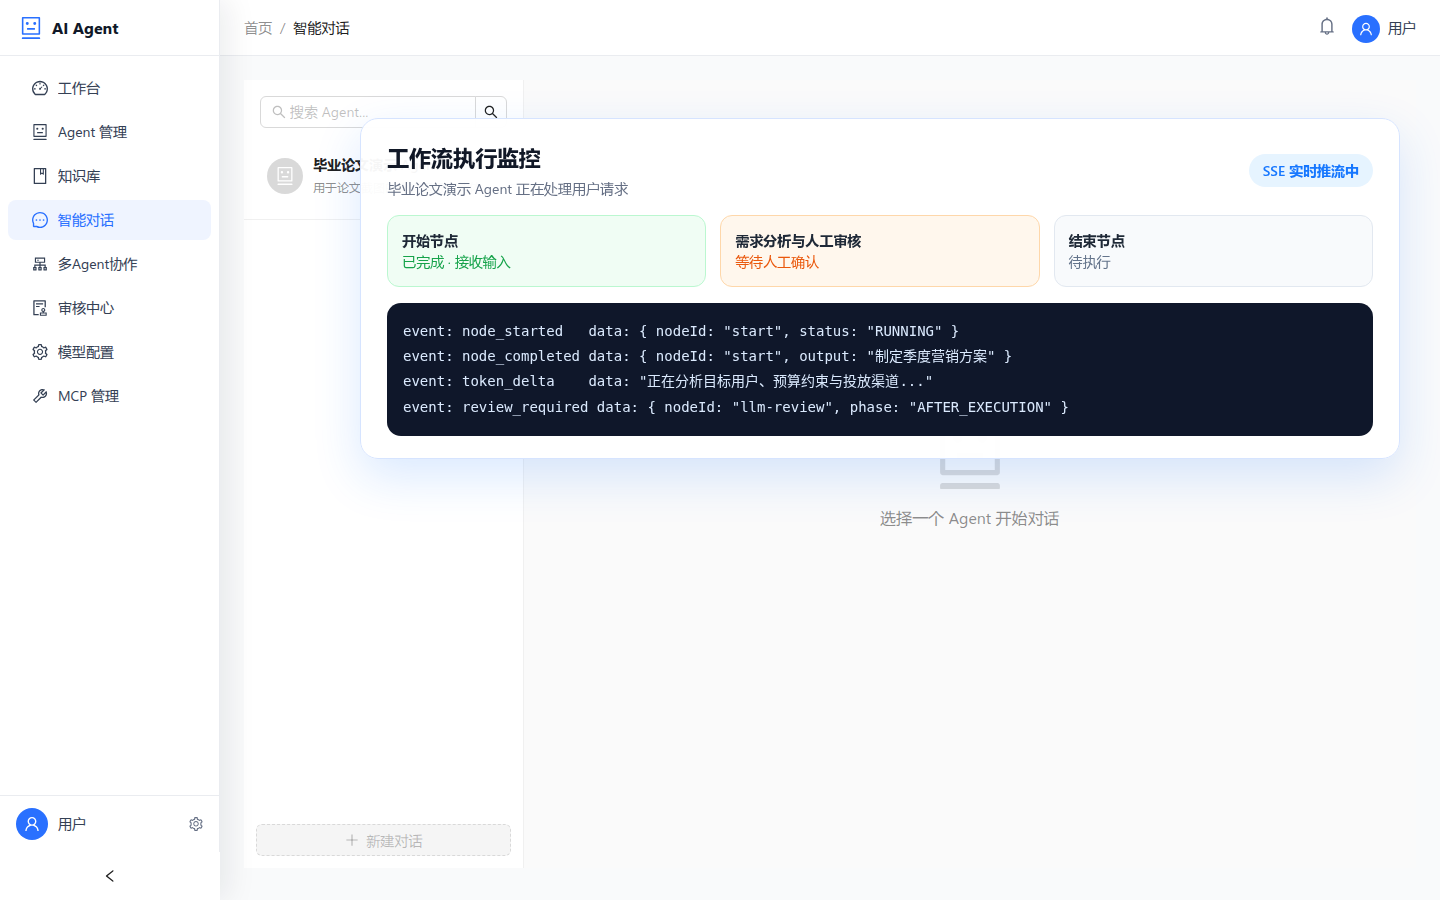
\includegraphics[width=1.0\textwidth]{figures/fig_wf_exec.png}
  \caption{工作流执行界面}
  \label{fig:wf_exec}
\end{figure}

\subsection{DAG 调度核心模块（Execution 聚合根）}

\subsubsection{（1）实现过程}

\texttt{Execution} 是工作流领域的聚合根，负责管理节点状态、执行上下文和整体状态流转。
每个节点完成后，调度器调用 \texttt{advance(nodeId, result)} 写入节点状态与输出，
并根据结果判断是否需要条件分支剪枝、人工检查点暂停或继续推进后继节点。

在计算后继节点时，\texttt{getReadyNodes()} 会结合有效入度判断可运行节点；
已完成、已跳过或已失败的节点不再阻塞其后继节点，因此系统可以自动调度所有依赖已满足的节点并行执行。

\subsubsection{（2）关键代码}

代码4-6展示了 \texttt{Execution.advance()} 的完整逻辑：

\begin{lstlisting}[language=Java, caption={代码4-6 Execution.advance() -- DAG 调度推进关键代码}]
public List<Node> advance(String nodeId, NodeExecutionResult result) {
    nodeStatuses.put(nodeId, result.getStatus());

    if (result.getOutputs() != null) {
        context.setNodeOutput(nodeId, result.getOutputs());
    }

    if (result.isRouting()) {
        pruneUnselectedBranches(nodeId, result.getSelectedBranchId());
    }

    if (result.isPaused()) {
        this.status = ExecutionStatus.PAUSED_FOR_REVIEW;
        this.pausedNodeId = nodeId;
        this.pausedPhase = result.getTriggerPhase();
        this.version++;
        return Collections.emptyList();
    }

    this.version++;

    if (isCompleted()) {
        this.status = ExecutionStatus.SUCCEEDED;
        return Collections.emptyList();
    }
    if (hasFailed()) {
        this.status = ExecutionStatus.FAILED;
        return Collections.emptyList();
    }

    return getReadyNodes();
}
\end{lstlisting}

代码4-7展示了条件分支剪枝的递归逻辑：

\begin{lstlisting}[language=Java, caption={代码4-7 Execution.skipNodeRecursively() -- 条件分支路径剪枝}]
private void skipNodeRecursively(String nodeId) {
    if (nodeStatuses.get(nodeId) != ExecutionStatus.PENDING) { return; }
    nodeStatuses.put(nodeId, ExecutionStatus.SKIPPED);

    Set<Node> successors = graph.getSuccessors(nodeId);
    for (Node successor : successors) {
        Set<Node> predecessors = graph.getPredecessors(successor.getNodeId());
        if (predecessors.size() <= 1) {
            skipNodeRecursively(successor.getNodeId());
        } else {
            boolean allSkipped = predecessors.stream().allMatch(
                pred -> nodeStatuses.get(pred.getNodeId())
                    == ExecutionStatus.SKIPPED);
            if (allSkipped) {
                skipNodeRecursively(successor.getNodeId());
            }
        }
    }
}
\end{lstlisting}

\subsubsection{（3）界面展示}

\begin{figure}[H]
  \centering
  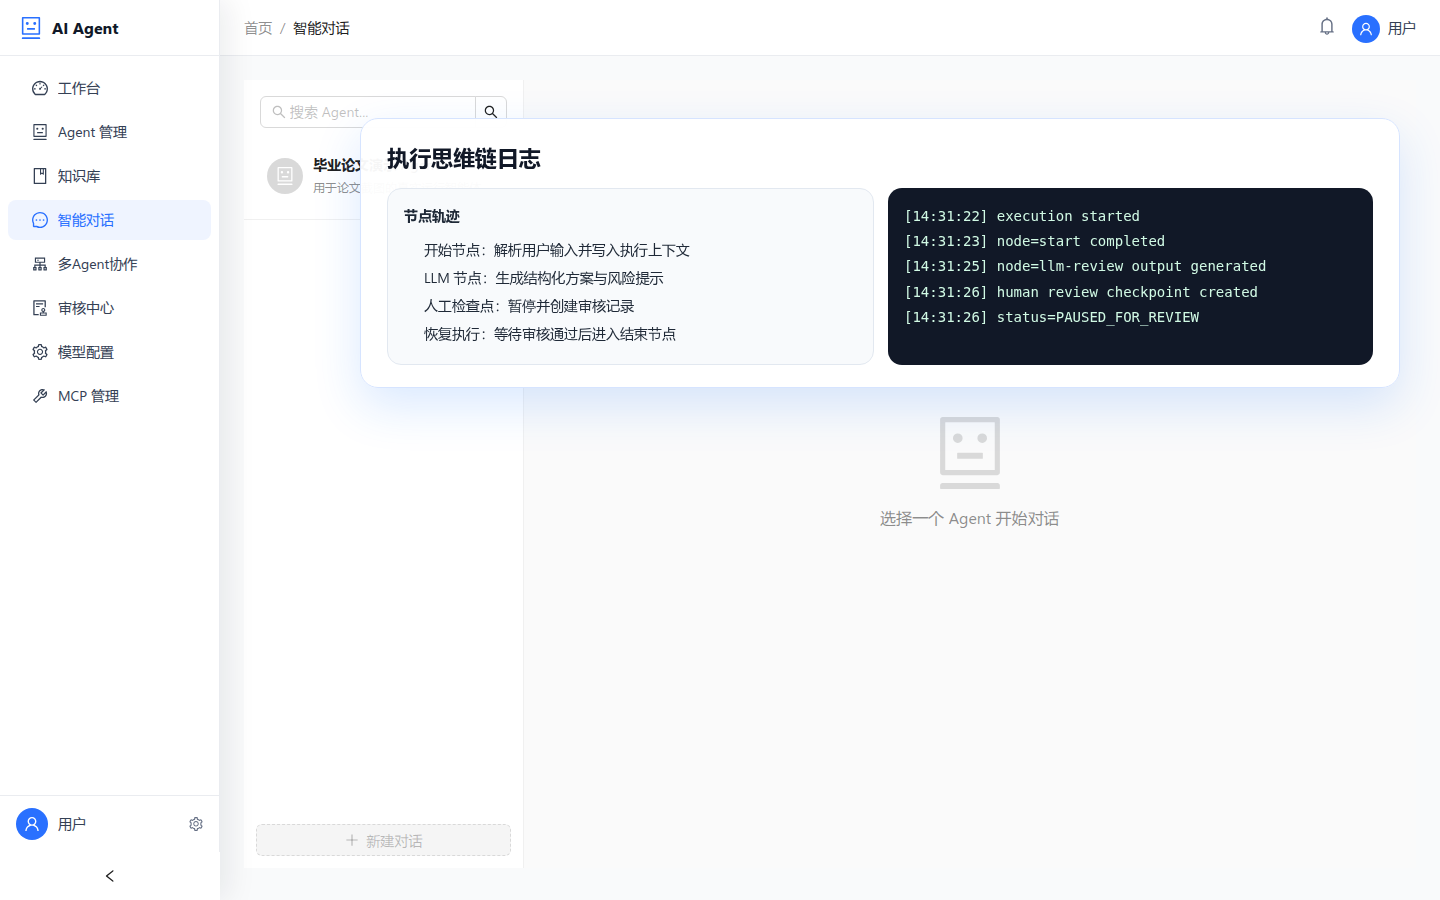
\includegraphics[width=0.88\textwidth]{figures/fig_wf_log.png}
  \caption{执行思维链日志}
  \label{fig:wf_log}
\end{figure}

\subsection{节点执行器策略模式}

\subsubsection{（1）实现过程}

系统采用\textbf{策略模式}解耦各节点类型的执行逻辑。
定义统一接口 \texttt{NodeExecutorStrategy}，
每种节点类型（LLM、CONDITION、KNOWLEDGE、TOOL、START、END）各自实现一个策略类，
注册到 \texttt{NodeExecutorFactory} 中统一管理。

调度器在收到待执行节点后，通过 \texttt{executorFactory.getStrategy(node.getType())}
获取对应策略，调用 \texttt{executeAsync()} 异步执行。
新增节点类型只需实现接口并注册，无需修改调度核心代码，满足开闭原则。

\subsubsection{（2）关键代码}

\begin{lstlisting}[language=Java, caption={代码4-8 NodeExecutorStrategy 接口定义}]
public interface NodeExecutorStrategy {
    CompletableFuture<NodeExecutionResult> executeAsync(
        Node node,
        Map<String, Object> resolvedInputs,
        StreamPublisher streamPublisher);

    NodeType getSupportedType();
}
\end{lstlisting}

\section{人工检查点与工作流恢复机制}

\subsection{人工检查点触发模块}

\subsubsection{（1）实现过程}

人工检查点（Human Checkpoint）用于在高风险节点执行前后引入人工审批。
调度器在节点执行前后调用 \texttt{checkPause()}，根据节点配置、触发阶段和已审核标记判断是否需要暂停。

当检查点条件满足时，系统在分布式锁保护下将执行状态更新为 \texttt{PAUSED\_FOR\_REVIEW}，
记录暂停节点和触发阶段，并将执行编号写入 Redis 待审批队列。
随后系统通过 SSE 推送 \texttt{workflow\_paused} 事件，前端据此展示审批弹窗。

系统支持两种触发阶段，其语义差异如表~\ref{tab:trigger_phase}~所示。

\begin{table}[H]
  \centering
  \caption{人工检查点两种触发阶段对比}
  \label{tab:trigger_phase}
  \begin{tabular}{lll}
    \toprule
    \textbf{维度} & \textbf{BEFORE\_EXECUTION} & \textbf{AFTER\_EXECUTION} \\
    \midrule
    触发时机 & 节点执行前 & 节点执行后 \\
    节点是否已执行 & 否 & 是 \\
    审批人可修改内容 & 节点输入（edits → SharedState） & 节点输出（覆盖 nodeOutput） \\
    审批通过后节点行为 & 重新执行节点 & 跳过执行，直接推进后续节点 \\
    典型场景 & 高风险操作预审（发送邮件前） & AI 输出内容人工校正 \\
    \bottomrule
  \end{tabular}
\end{table}

\subsubsection{（2）关键代码}

\begin{lstlisting}[language=Java, caption={代码4-9 SchedulerService.checkPause() -- 人工检查点触发判断}]
private boolean checkPause(String executionId, Node node,
        TriggerPhase phase, StreamPublisher publisher,
        Map<String, Object> outputs) {

    HumanReviewConfig config = node.getHumanReviewConfig();
    if (config == null || !config.isEnabled()) { return false; }
    if (config.getTriggerPhase() != phase) { return false; }

    Execution execution = executionRepository.findById(executionId)
        .orElseThrow();
    if (execution.isNodeReviewed(node.getNodeId())) { return false; }

    String lockKey = "lock:exec:" + executionId;
    RLock lock = redisService.getLock(lockKey);
    try {
        lock.lock(30, TimeUnit.SECONDS);
        NodeExecutionResult pausedResult =
            NodeExecutionResult.paused(phase, outputs);
        execution.advance(node.getNodeId(), pausedResult);
        executionRepository.update(execution);
        humanReviewQueuePort.addToPendingQueue(executionId);
        publisher.publishEvent("workflow_paused", Map.of(...));
    } finally {
        if (lock.isHeldByCurrentThread()) { lock.unlock(); }
    }
    return true;
}
\end{lstlisting}

\subsubsection{（3）界面展示}

当工作流执行到配置了人工检查点的节点时，
前端通过 SSE 接收 \texttt{workflow\_paused} 事件，弹出审批面板。
界面展示节点的输入（BEFORE 阶段）或输出（AFTER 阶段）内容，
审批人可视情况对字段进行修改，然后点击"通过"或"拒绝"。

\begin{figure}[H]
  \centering
  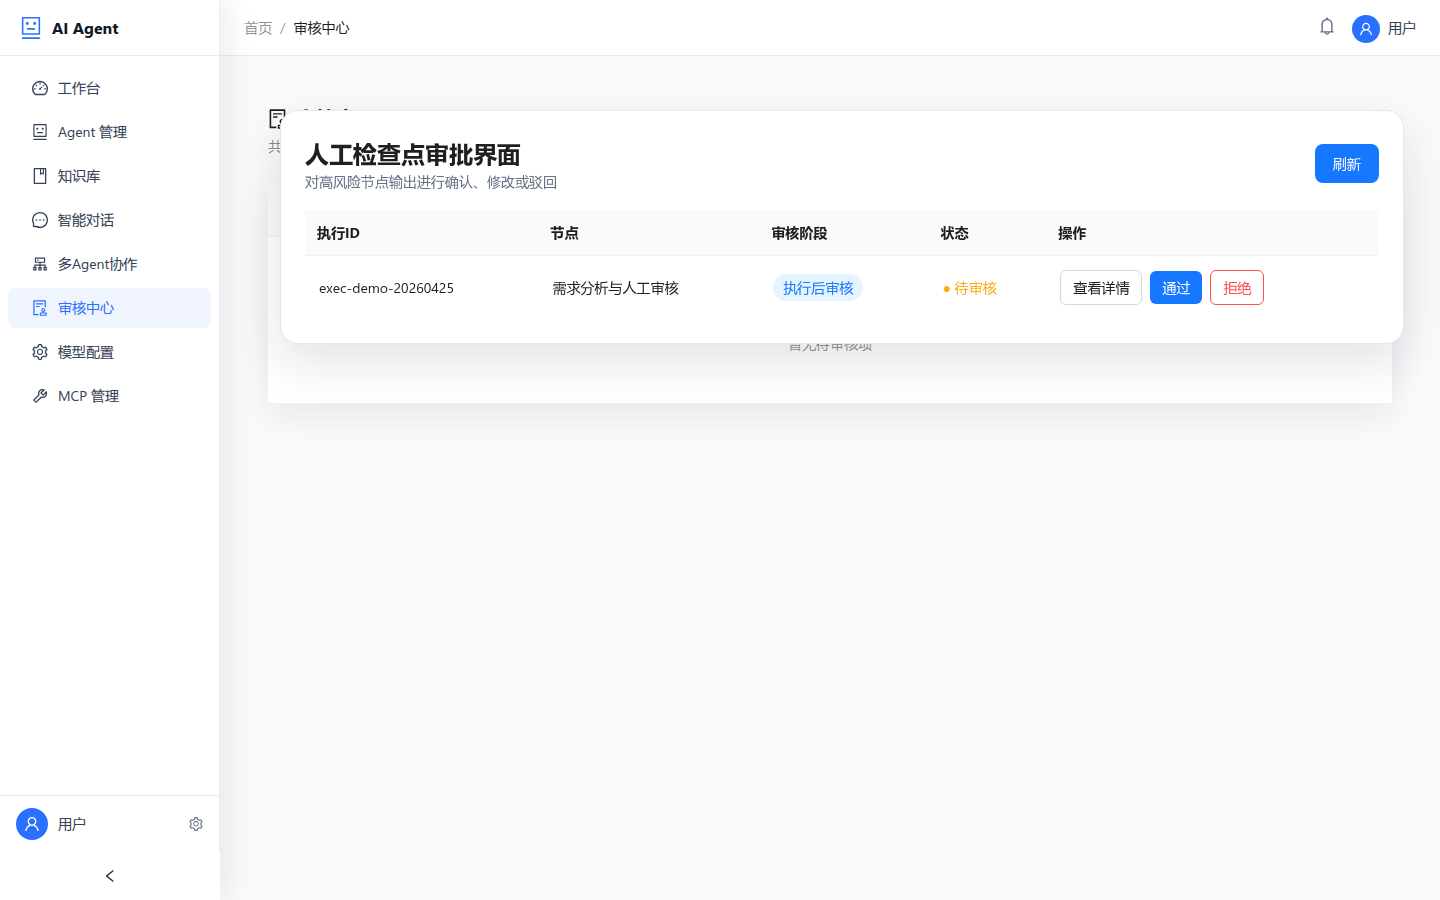
\includegraphics[width=0.92\textwidth]{figures/fig_review_panel.png}
  \caption{人工检查点审批界面}
  \label{fig:review_panel}
\end{figure}

\subsection{工作流恢复模块}

\subsubsection{（1）实现过程}

审批通过后，前端调用 \texttt{POST /api/workflow/reviews/resume} 接口并携带执行编号、暂停节点、
乐观锁版本号以及可选编辑内容。服务端在分布式锁内校验暂停节点和版本号，
防止重复审批或并发恢复导致状态不一致。

恢复过程中，系统会根据暂停阶段合并审批人修改的数据，写入审核记录，
调用 \texttt{execution.resume()} 将工作流恢复为运行态，并从 Redis 待审批队列移除该执行。
若暂停发生在节点执行后，调度器直接推进后继节点；若暂停发生在节点执行前，则重新调度当前节点执行。

\subsubsection{（2）关键代码}

\begin{lstlisting}[language=Java, caption={代码4-10 SchedulerService.resumeExecution() -- 工作流恢复关键代码}]
public void resumeExecution(String executionId, String nodeId,
        Integer expectedVersion, Map<String, Object> edits,
        Long reviewerId, String comment, Map<String, Map<String, Object>> nodeEdits) {
    RLock lock = redisService.getLock("lock:exec:" + executionId);
    try {
        lock.lock(30, TimeUnit.SECONDS);
        Execution execution = executionRepository.findById(executionId).orElseThrow();
        if (!pausedNode(execution, nodeId)) { return; }
        if (expectedVersion != null && !expectedVersion.equals(execution.getVersion())) {
            throw new OptimisticLockingFailureException("版本冲突");
        }

        TriggerPhase phase = defaultPhase(execution.getPausedPhase());
        mergeReviewEdits(execution, nodeId, edits, nodeEdits, phase);
        humanReviewRepository.save(buildApproveRecord(executionId, nodeId, reviewerId, phase, comment));

        List<Node> readyNodes = execution.resume(nodeId, edits);
        executionRepository.update(execution);
        humanReviewQueuePort.removeFromPendingQueue(executionId);
        publishAndSchedule(executionId, nodeId, readyNodes, phase, edits);
    } finally {
        if (lock.isHeldByCurrentThread()) { lock.unlock(); }
    }
}
\end{lstlisting}

\subsubsection{（3）界面展示}

审批人点击"通过"后，前端通过 SSE 接收 \texttt{workflow\_resumed} 事件，
画布中暂停的节点恢复执行，执行日志继续滚动追加。

\begin{figure}[H]
  \centering
  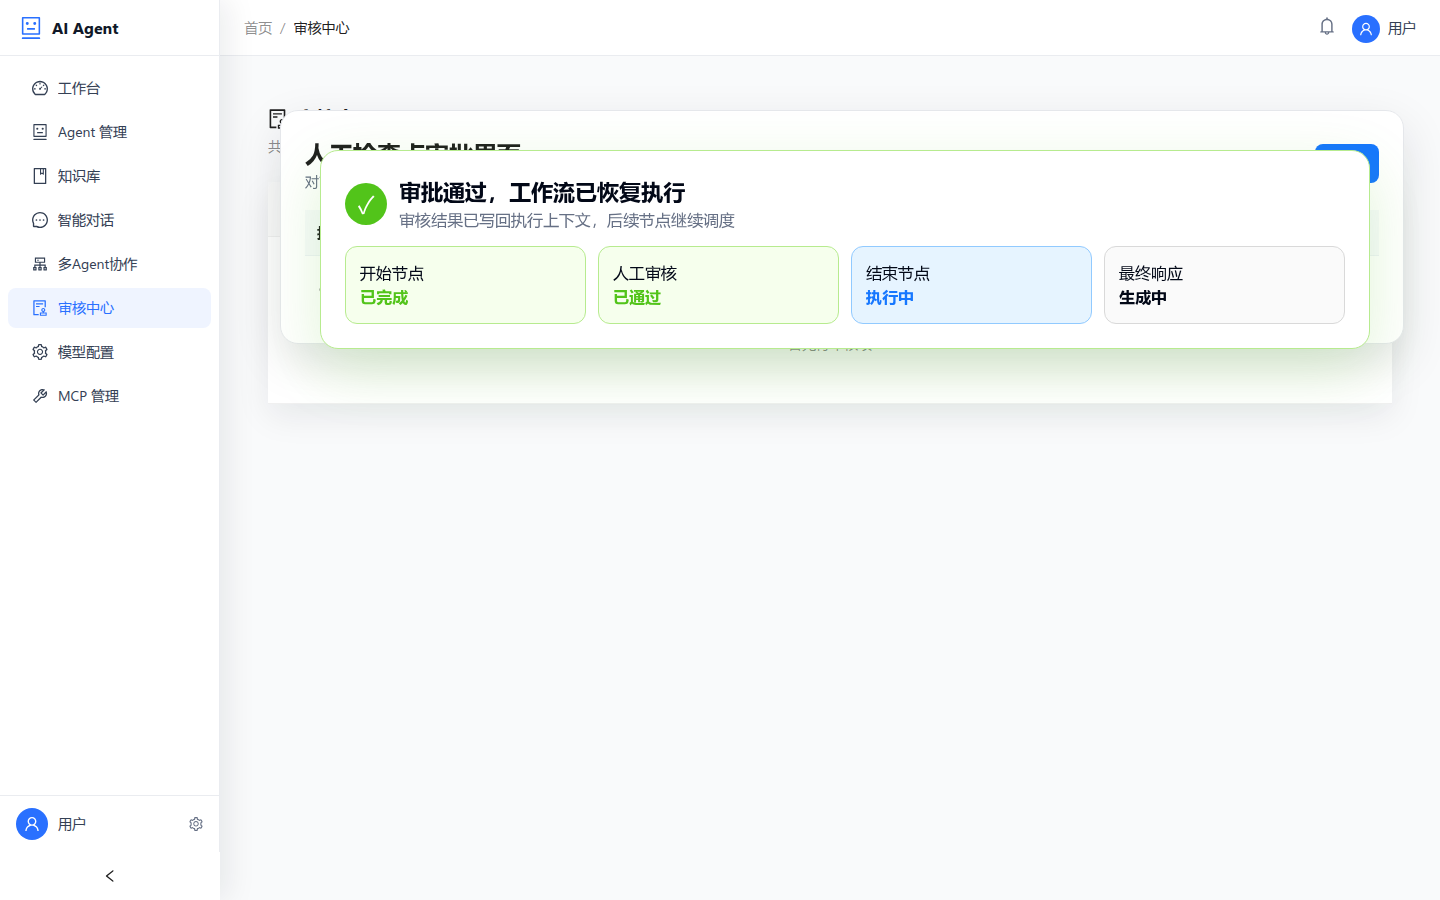
\includegraphics[width=0.85\textwidth]{figures/fig_resume_ui.png}
  \caption{审批通过后工作流恢复执行界面}
  \label{fig:resume_ui}
\end{figure}

\subsection{并发安全保障}

\subsubsection{（1）实现过程}

多人同时对同一暂停中的工作流进行审批操作时，若无任何保护机制，
则可能导致多次状态转换、多次提交或数据不一致。
本系统通过以下两层机制保障并发安全：

\textbf{分布式锁（Redis Redisson）：}
所有 \texttt{pause / resume / reject} 操作均在 \texttt{lock:exec:\{executionId\}}
锁的保护下执行，锁超时设置为 30 秒，确保同一时刻只有一个线程可以修改执行状态。

\textbf{乐观锁（executionVersion）：}
\texttt{Execution} 聚合根维护 \texttt{version} 字段，
每次状态变更（\texttt{advance()} / \texttt{resume()} / \texttt{reject()}）均令其自增。
前端在发起审批请求时必须携带当前 \texttt{version}，
服务端比较 \texttt{expectedVersion} 与数据库中的 \texttt{version}，
若不一致（代表已被他人提前操作）则抛出 \texttt{OptimisticLockingFailureException}，
HTTP 层返回 \textbf{409 Conflict}，前端提示重新加载。

\subsubsection{（2）关键代码}

\begin{lstlisting}[language=Java, caption={代码4-11 Execution.java -- 乐观锁版本控制}]
@Builder.Default
private Integer version = 0;

public List<Node> resume(String nodeId, Map<String, Object> inputs) {
    this.status = ExecutionStatus.RUNNING;
    this.pausedNodeId = null;
    this.pausedPhase = null;
    this.version++;
    this.reviewedNodes.add(nodeId);
}
\end{lstlisting}

\section{知识库与检索增强实现}

\subsection{知识数据集与文档接入流程}

\subsubsection{（1）实现过程}

知识库模块用于为工作流中的知识节点和 LLM 节点提供外部知识支撑。
接口层通过 \texttt{KnowledgeController} 提供数据集创建、文档上传、查询、删除和检索接口；
应用层由 \texttt{KnowledgeApplicationService} 串联文件校验、对象存储、文档记录入库和异步处理。

用户上传文档时，系统先完成数据集归属校验和文件合法性校验，再将原始文件保存到 MinIO，
同时创建状态为 \texttt{PENDING} 的文档记录。随后应用层触发异步文档处理任务，
使上传接口可以快速返回，避免解析和向量化等耗时操作阻塞前端请求。

\subsubsection{（2）关键代码}

代码4-12展示了文档上传和异步处理入口的关键逻辑：

\begin{lstlisting}[language=Java, caption={代码4-12 KnowledgeApplicationService -- 文档上传与异步处理}]
@Transactional
public KnowledgeDocument uploadDocument(Long userId, String datasetId,
        MultipartFile file, ChunkingConfig chunkingConfig) {
    KnowledgeDataset dataset = datasetRepository.findById(datasetId).orElseThrow();
    validateOwnership(userId, dataset.getCreatedBy());

    fileValidator.validate(file);
    String fileUrl = fileStorageService.upload(bucketName, objectName,
        file.getInputStream(), file.getContentType());

    KnowledgeDocument document = KnowledgeDocument.pending(
        datasetId, file.getOriginalFilename(), fileUrl, chunkingConfig);
    documentRepository.save(document);

    dataset.addDocument();
    datasetRepository.save(dataset);
    asyncDocumentProcessor.processDocumentAsync(document);
    return document;
}
\end{lstlisting}

\subsubsection{（3）界面展示}

用户可在知识库页面中创建数据集、上传文档并查看文档处理状态。
当前端轮询或刷新列表时，可看到文档从待处理、处理中到已完成的状态变化。

\begin{figure}[H]
  \centering
  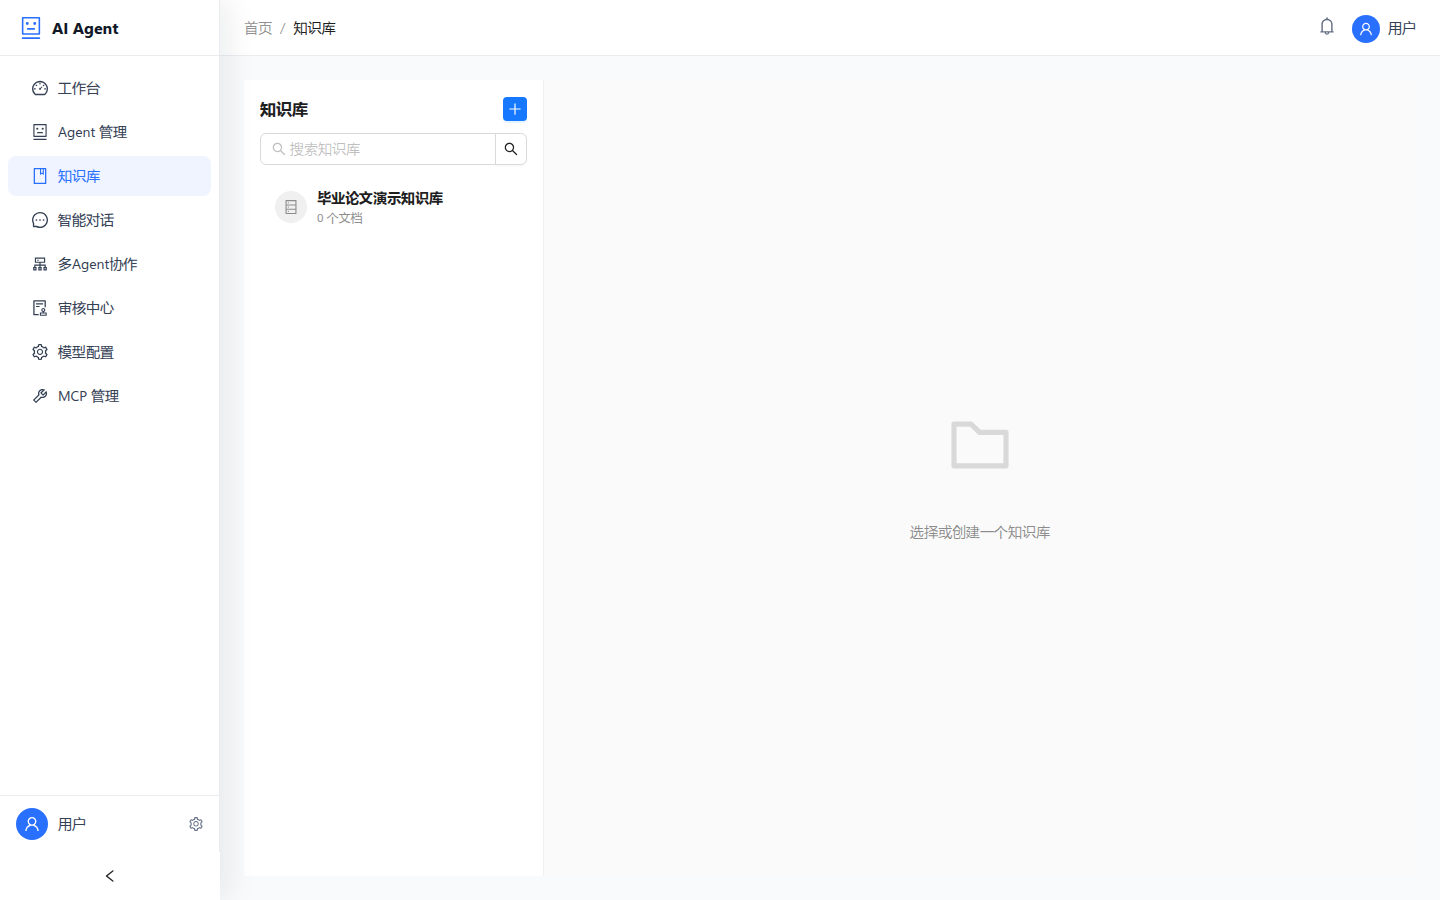
\includegraphics[width=0.92\textwidth]{figures/fig_knowledge_ui.png}
  \caption{知识库管理界面}
  \label{fig:knowledge_ui}
\end{figure}

\subsection{异步分块、向量化与检索增强}

\subsubsection{（1）实现过程}

异步文档处理器承担知识接入链路中的核心计算任务，整体流程为
"对象存储下载 → 文档解析 → 文本分块 → 批量向量化存储 → 状态回写"。
处理器先将文档状态更新为 \texttt{PROCESSING}，再通过 \texttt{DocumentReaderPort} 解析 PDF、Word、Markdown 等文件，
并按照 \texttt{ChunkingConfig} 调用 \texttt{TextSplitterPort} 完成文本分块。

分块完成后，系统为每个文本块构造向量文档和元数据，按批次写入 Milvus。
运行时，工作流或检索接口可根据用户问题进行语义召回，并将召回结果作为知识上下文注入 LLM 节点输入，
实现检索增强生成。

\subsubsection{（2）关键代码}

代码4-13展示了异步文档处理与批量向量化的关键实现：

\begin{lstlisting}[language=Java, caption={代码4-13 AsyncDocumentProcessor -- 文档分块与向量化处理}]
@Async
public void processDocumentAsync(KnowledgeDocument document) {
    document.startProcessing();
    documentRepository.save(document);

    InputStream fileStream = fileStorageService.download(bucketName,
        extractObjectName(document.getFileUrl()));
    List<String> parsedTexts = documentReaderPort.readDocument(
        fileStream, document.getFilename());

    ChunkingConfig config = document.getChunkingConfig().normalized();
    List<String> chunks = textSplitterPort.split(parsedTexts, config);

    List<Document> batch = buildVectorDocuments(document, chunks);
    vectorStore.addDocuments(batch);

    document.markCompleted();
    documentRepository.save(document);
}
\end{lstlisting}

代码4-14展示了基于向量数据库的检索增强接口：

\begin{lstlisting}[language=Java, caption={代码4-14 MilvusVectorStoreAdapter -- 知识检索接口}]
public List<String> searchKnowledge(String query, Long agentId, int topK) {
    SearchRequest request = SearchRequest.query(query)
        .withTopK(topK)
        .withFilterExpression("agent_id == " + agentId);
    return springAiVectorStore.similaritySearch(request).stream()
        .map(Document::getText)
        .toList();
}
\end{lstlisting}

\subsubsection{（3）界面展示}

知识检索结果可直接服务于工作流中的知识节点，也可在前端页面中用于展示数据集命中文档摘要，
帮助用户理解知识增强的来源与效果。

\section{SSE 全链路实时推流实现}

\subsection{（1）实现过程}

系统采用 Server-Sent Events（SSE）实现工作流执行过程的全链路实时推流，
涵盖节点执行状态变更、LLM 流式输出增量片段（delta）、人工检查点暂停/恢复等事件。

\texttt{StreamPublisher} 是流推送的抽象接口，
由 \texttt{StreamPublisherFactory} 根据 \texttt{StreamContext}（含 executionId、nodeId）
创建对应的 \texttt{SseStreamPublisher} 实例。每个 SSE 连接通过 \texttt{executionId}
注册到 Spring \texttt{SseEmitter} 池中，连接建立时推送 \texttt{connected} 事件，
之后调度器在每个关键时刻通过 \texttt{publisher.publishEvent(type, payload)} 推送对应事件。

系统内置心跳机制，每 15 秒推送一次 \texttt{ping} 事件防止浏览器端超时关闭连接。

\subsection{（2）关键代码}

\begin{lstlisting}[language=Java, caption={代码4-15 StreamPublisher 接口 -- SSE 推流核心方法}]
public interface StreamPublisher {
    void publishStart();
    void publishDelta(String delta);
    void publishFinish(NodeExecutionResult result);
    void publishEvent(String eventType, Map<String, Object> payload);
}
\end{lstlisting}

\subsection{（3）界面展示}

前端基于 SSE 事件流实时驱动三个区域的更新：
左侧工作流画布（节点颜色实时变化）、中间流式输出区（LLM delta 逐字追加）、
右侧思维链日志面板（节点执行时序和输入/输出）。

\begin{figure}[H]
  \centering
  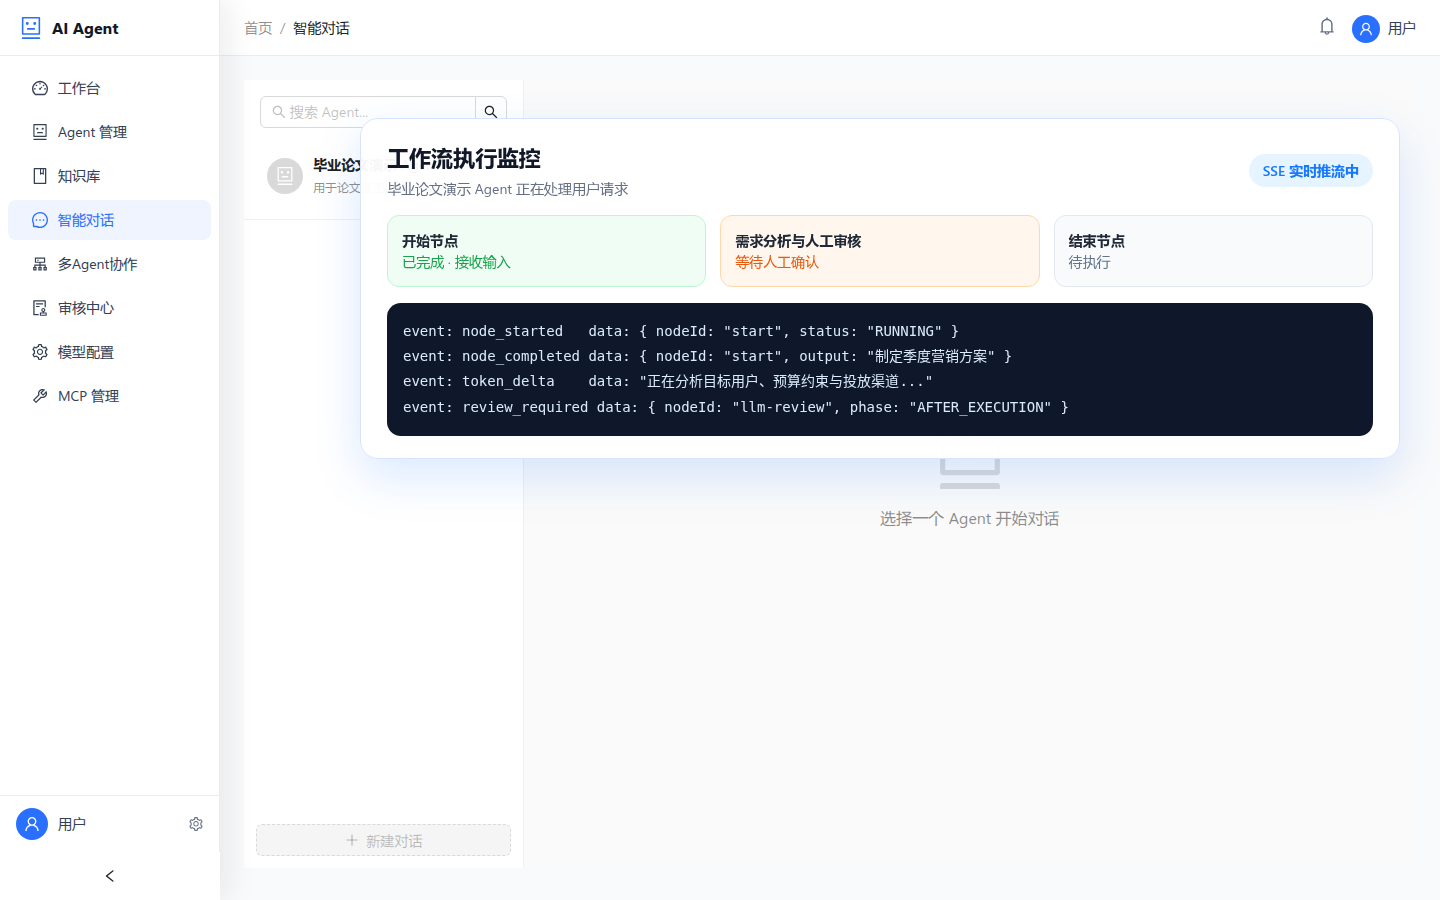
\includegraphics[width=0.92\textwidth]{figures/fig_sse_ui.png}
  \caption{SSE 实时推流前端展示}
  \label{fig:sse_ui}
\end{figure}

\section{本章小结}

本章围绕论文确定的五个核心模块，系统介绍了用户认证与系统安全支撑、Agent 管理与可视化编排、
工作流调度执行、人工检查点与工作流恢复、知识库与检索增强的实现过程，
并补充说明了 SSE 全链路实时推流对前端交互体验的支撑作用。

在用户认证模块中，系统实现了注册、登录、找回密码、验证码校验与访问安全控制，
为平台各项业务能力提供统一身份基础；在 Agent 管理模块中，系统通过 \texttt{graphJson}
将可视化画布与运行时工作流图定义打通，并借助版本快照实现了发布与回滚；
在工作流调度模块中，\texttt{Execution} 聚合根通过 \texttt{advance()} 和有效入度计算
实现无依赖节点的自动并行与状态推进；
在人工审核模块中，系统通过两阶段检查点、Redis 分布式锁与乐观锁版本号保障暂停、审批与恢复的可靠执行。

在知识库模块中，系统实现了从文档上传、对象存储、异步分块、批量向量化到检索增强的完整闭环。
最后，SSE 推流机制将执行进度、审核状态和流式结果实时反馈给前端，
形成了从配置、执行到交互回看的完整用户链路。
